\documentclass[a4paper,twoside,12pt]{memoir}

\usepackage[T1]{fontenc}
\usepackage[utf8]{inputenc}
\usepackage[margin=2.5cm]{geometry}
\usepackage{arara}

\addbibresource{references.bib}
\newcommand{\araraversion}{4.0}
\newcommand{\todo}[1]{\fbox{\em#1}}

\begin{document}

\begin{titlingpage}
\vspace*{2em}

\begin{center}

\includegraphics[scale=0.7]{../logos/logo2.pdf}

\vspace{4em}

\begin{tcolorbox}[
  boxrule=0pt,
  colback=araracolour,
  top=1em,
  bottom=1em
]
  \color{white}
  \centering
  \Huge
  \sffamily
  \bfseries User manual
\end{tcolorbox}

\vspace{6em}

{\large\em Paulo Cereda, Marco Daniel,\\
Brent Longborough, and Nicola Talbot\par}

\vspace{2em}

\url{https://github.com/cereda/arara}

\vfill

{\color{araracolour}
\LARGE
\sffamily
\bfseries
Version \araraversion}

\end{center}
\end{titlingpage}

\chapterstyle{araraheadings}
\pagestyle{headings}
\frontmatter
\nouppercaseheads

\cleardoublepage

\vspace*{25em}

\begin{flushright}
\em No birds were harmed in the making of this manual.
\end{flushright}

% !TeX root = ../arara-manual.tex
\chapter*{Foreword}
\label{chap:foreword}

\epigraph{That deserves no less than a ``Holy guacamole!''.}{\textsc{Gonzalo Medina}}

{\setlength{\parskip}{1em}
Creating a PDF from \LaTeX\ code can be quite tiresome. Suppose I am using \TeX works and I have a document that has a bibliography, glossary and index, then I need to select the \rbox{pdflatex} tool and click on the typeset button, then select the \rbox{bibtex} tool and click on the typeset button, then select the \rbox{makeindex} tool and click on the typeset button, then select the \rbox{makeglossaries} tool (which I may need to add first) and click on the typeset button, then select the \rbox{pdflatex} tool and click on the typeset button, and once more to ensure all the cross-references are up to date. Then I edit the document and have to go through that whole process all over again!

Automation makes life so much simpler. Instead of all those tools that I need to keep selecting, I just need one tool, in this case \arara, which will do all the necessary work for me behind the scenes.

Some automation tools try to be clever, but there are invariably exceptions that trip them up. \arara\ does not try to be clever; it just does what it is told to do. The instructions are provided as special comments in the source code that \TeX\ ignores, but they are human-readable and can also provide a hint to non-\arara\ co-authors as to what tools are required in order to complete the document build.

The new improved \arara\ version 4.0 now comes with some exciting features, such as the ability to use conditionals, and it definitely ranks as my favourite automation tool for document creation. Paulo has done a great job, and I would like to take this opportunity to thank
him for his patience in dealing with my many feature requests!}

\vfill

\begin{flushright}
Nicola Louise Cecilia Talbot\\
\emph{on behalf of the \arara\ team}
\end{flushright}

% !TeX root = ../arara-manual.tex
\chapter*{Prologue}
\label{chap:prologue}

\epigraph{Moral of the story: never read the
documentation, bad things happen.}{\textsc{David Carlisle}}

{\setlength{\parskip}{1em}
Writing software is easy. Writing \emph{good} software is extremely difficult. When the counter stopped at version 3.0, Brent, Marco and I decided it was time for \arara\ to graduate and finally be released in \TeX\ Live. My life had changed.

It was a success. A lot of people liked the idea of explicitly telling our tool how to compile their \TeX\ dcouments instead of relying on guesswork. It was indeed a cool concept! But then, the inevitable happened: a lot of bugs had emerged from the dark depths of my humble code.

In all seriousness, \emph{I was about to give up}. My code was not awful, but there were a couple of critical and blocking bugs. Something very drastic had to be done in order to put \arara\ back on track. Then, walking on faith, I decided to rewrite the tool entirely from scratch. In order to achieve this goal, I created a \href{https://github.com/cereda/nightingale}{sandbox} and started working on the new code.

It was my redemption. Nicola helped me with the new version, writing code, fixing bugs and suggesting new features. Soon, we all achieved a very pleasant result. It was like \arara\ was about to hatch again. Version 4.0 was definitely at our hands. Now, it is up to you.

Surprisingly, this humble user manual is not the best resource for learning about our tool. If you really want to see \arara\ in action, I strongly recommend \href{https://www.dickimaw-books.com/latex/admin}{\LaTeX\ for administrative work}, an amazing book freely available for download. The author is, of course, Nicola herself! She explains how \LaTeX\ can be used for administrative work, such as writing correspondence, performing repetitive tasks or typesetting problem sheets on exam papers. And \arara\ is there!

Enjoy the new version. Happy \TeX ing with \arara!
\par}

\vfill

\begin{flushright}
Paulo Roberto Massa Cereda\\
\emph{on behalf of the \arara\ team}
\end{flushright}

\chapter*{Release information}
\label{chap:releaseinformation}

\epigraph{Are there programming languages other
than \TeX?}{\textsc{Enrico Gregorio}}

\emph{Release information here}

\chapter*{Licenses}
\label{chap:license}

\epigraph{Anything that prevents you from being friendly, a good neighbour, is a terror tactic.}{\textsc{Richard Stallman}}

\section*{Application}
\label{sec:licenseapplication}

The main application is licensed under the \href{http://www.opensource.org/licenses/bsd-license.php}{New BSD License}. It is important to observe that the New BSD License has been verified as a GPL-compatible free software license by the \href{http://www.fsf.org/}{Free Software Foundation}, and has been vetted as an open source license by the \href{http://www.opensource.org/}{Open Source Initiative}.

\vspace{1em}

\begin{messagebox}{New BSD License}{araracolour}{\icinfo}{white}

\includegraphics[scale=0.25]{../logos/logo1.pdf}

Copyright \textcopyright\ 2012--2018, Paulo Roberto Massa Cereda\\
All rights reserved.

\vspace{1em}

Redistribution and use in source and binary forms, with or without modification, are permitted provided that the following conditions are met:

\begin{itemize}
\item Redistributions of source code must retain the above copyright notice, this list of conditions and the following disclaimer.

\item Redistributions in binary form must reproduce the above copyright notice, this list of conditions and the following disclaimer in the documentation and/or other materials provided with the distribution.
\end{itemize}

This software is provided by the copyright holders and contributors ``as is'' and any express or implied warranties, including, but not limited to, the implied warranties of merchantability and fitness for a particular purpose are disclaimed. In no event shall the copyright holder or contributors be liable for any direct, indirect, incidental, special, exemplary, or consequential damages (including, but not limited to, procurement of substitute goods or services; loss of use, data, or profits; or business interruption) however caused and on any theory of liability, whether in contract, strict liability, or tort (including negligence or otherwise) arising in any way out of the use of this software, even if advised of the possibility of such damage.
\end{messagebox}

\section*{Helper tools}
\label{sec:licensehelpertools}

During the build phase, two tools were developed in order to ease writing and checking of rules and language files (both tools are available in the \abox[araracolour]{tools/} directory of our repository). These tools are licensed under the \href{https://opensource.org/licenses/MIT}{MIT license}.

\vspace{1em}

\begin{messagebox}{MIT License}{araracolour}{\icinfo}{white}
\setlength{\parskip}{1em}
\textbf{Rule and language helper tools}\\
Copyright \textcopyright\ 2012--2018, Paulo Roberto Massa Cereda\\
All rights reserved.

Permission is hereby granted, free of charge, to any person obtaining a copy of this software and associated documentation files (the ``Software''), to deal in the Software without restriction, including without limitation the rights to use, copy, modify, merge, publish, distribute, sublicense, and/or sell copies of the Software, and to permit persons to whom the Software is furnished to do so, subject to the following conditions:

The above copyright notice and this permission notice shall be included in all copies or substantial portions of the Software.

The software is provided ``as is, without warranty of any kind, express or implied, including but not limited to the warranties of merchantability, fitness for a particular purpose and noninfringement. In no event shall the authors or copyright holders be liable for any claim, damages or other liability, whether in an action of contract, tort or otherwise, arising from, out of or in connection with the software or the use or other dealings in the software.
\end{messagebox}

\section*{Visual identity}
\label{sec:licensevisualidentity}

The official \arara\ logos constitute the visual identity of our tool and can be used and distributed under \href{https://creativecommons.org/licenses/by-nd/4.0/}{Creative Commons BY-ND 4.0}. The following elements are availalbe in the \abox[araracolour]{logos/} directory of our repository as PDF files:

\begin{tcolorbox}[
  enhanced jigsaw,
  opacityupper=1.0,
  opacityback=.60,
  interior style={
    pattern=checkerboard light gray
  },
  drop lifted shadow,
  colback=araracolour!5,
  colframe=araracolour,
  breakable,
  toptitle=0.2em,
  bottomtitle=.2em,
  before skip=1em,
  after skip=1.4em]
\centering
{\setlength{\tabcolsep}{30pt}
\begin{tabular}{ccc}

\includegraphics[scale=.15]{../logos/logo1.pdf} &

\includegraphics[scale=.15]{../logos/logo2.pdf} &

\includegraphics[scale=.15]{../logos/bird.pdf} \\[.5em]
Horizontal version &
Vertical version &
Parrot only \\[.5em]
\abox[araracolour]{logo1.pdf} &
\abox[araracolour]{logo2.pdf} &
\abox[araracolour]{bird.pdf}
\end{tabular}}
\end{tcolorbox}

\begin{messagebox}{Creative Commons BY-ND 4.0}{araracolour}{\icinfo}{white}
\setlength{\parskip}{1em}

This is a human-readable summary of (and not a substitute for) the license. You are free to:

\textbf{Share} -- copy and redistribute the material in any medium or format for any purpose, even commercially. The licensor cannot revoke these freedoms as long as you follow the license terms.

Under the following terms:

\textbf{Attribution} -- You must give appropriate credit, provide a link to the license, and indicate if changes were made. You may do so in any reasonable manner, but not in any way that suggests the licensor endorses you or your use.

\textbf{No derivatives} -- If you remix, transform, or build upon the material, you may not distribute the modified material.

\textbf{No additional restrictions} -- You may not apply legal terms or technological measures that legally restrict others from doing anything the license permits.

\textbf{Notices:}

You do not have to comply with the license for elements of the material in the public domain or where your use is permitted by an applicable exception or limitation.

No warranties are given. The license may not give you all of the permissions necessary for your intended use. For example, other rights such as publicity, privacy, or moral rights may limit how you use the material.

{\centering\color{araracolour}\scalebox{2.0}{\ccbynd}\par} 
\end{messagebox}


\cleardoublepage

\vspace*{25em}

\begin{flushright}
\em To Marco's son Niclas.
\end{flushright}

\cleardoublepage

\tableofcontents*

\cleardoublepage

\listoffigures*

\cleardoublepage

\listoftables*

\mainmatter

\part[A primer on formats and scripting]{A primer on\\ formats and scripting}
\label{part:primer}

% !TeX root = ../arara-manual.tex
\chapter{YAML}
\label{chap:yaml}

According to the \href{http://yaml.org/spec/1.2/spec.html}{specification}, YAML (a recursive acronym for \emph{YAML Ain't Markup Language}) is a human-friendly, cross language, Unicode-based data serialization language designed around the common native data type of programming languages. \arara\ uses this format in three circumstances:

\begin{enumerate}
% TODO: fix section reference
\item\emph{Parametrized directives}, as the set of attribute/value pairs (namely, argument name and corresponding value) is represented by a map. This particular type of directive is formally introduced in Section~\ref{foo} (page~\pageref{foo}).

% TODO: fix section reference
\item\emph{Rules}, as their entire structure is represented by a set of specific keys and their corresponding values (a proper YAML document). A rule follows a very strict model, detailed in Section~\ref{foo} (page~\pageref{foo}).

% TODO: fix section reference
\item\emph{Configuration files}, as the general settings are represented by a set of specific keys and their corresponding values (a proper YAML document). Configuration files are covered in Section~\ref{foo} (page~\pageref{foo}).
\end{enumerate}

This chapter only covers the relevant parts of the YAML format for a consistent use with \arara. For advanced topics, I highly recommend the complete format specification, available online.

\section{Collections}
\label{sec:yamlcollections}

According to the specification, YAML's block collections use indentation for scope and begin each entry on its own line. Block sequences indicate each entry with a dash and space. Mappings use a colon and space to mark each \emph{key: value} pair. Comments begin with an octothorpe. \arara\ relies solely on mappings and a few scalars to sequences at some point. Let us see an example of a sequence:

\begin{codebox}{A sequence of scalars in YAML}{teal}{\icnote}{white}
team:
- Paulo Cereda
- Marco Daniel
- Brent Longborough
- Nicola Talbot
\end{codebox}

It is quite straightforward: \abox{team} holds a sequence of four scalars. YAML also has flow styles, using explicit indicators rather than indentation to denote scope. The flow sequence is written as a comma-separated list within square brackets:

\begin{codebox}{A sequence of scalars in YAML}{teal}{\icnote}{white}
primes: [ 2, 3, 5, 7, 11 ]
\end{codebox}

Attribute maps are easily represented by nesting entries, respecting indentation. For instance, consider a map \abox{developer} containing two keys, \abox{name} and \abox{country}. The YAML representation is presented as follows:

\begin{codebox}{An attribute map in YAML}{teal}{\icnote}{white}
developer:
 name: Paulo
 country: Brazil
\end{codebox}

% TODO: fix section reference
Similarly, the flow mapping uses curly braces. Observe that this is the form adopted by a parametrized directive (see syntax on Section~\ref{foo}, page~\pageref{foo}):

\begin{codebox}{An attribute map in YAML (flow mapping)}{teal}{\icnote}{white}
developer: { name: Paulo, country: Brazil }
\end{codebox}

An attribute map can contain sequences as well. Consider the following code where \abox{developers} holds a list of two developers containing their names and countries:

\begin{codebox}{An attribute map with sequences in YAML}{teal}{\icnote}{white}
developers:
- name: Paulo
  country: Brazil
- name: Marco
  country: Germany
\end{codebox}

The previous code can be easily represented in flow style by using square and curly brackets to represent sequences and attribute maps.

\section{Scalars}
\label{sec:yamlscalars}

% TODO: fix section reference
Scalar content can be written in block notation, using a literal style, indicated by a vertical bar, where \emph{all line breaks are significant}. Alternatively, they can be written with the folded style, denoted by a greater-than sign, where \emph{each line break is folded to a space} unless it ends an empty or a more-indented line. It is mportant to note that \arara\ intensively uses both styles (as seen in Section~\ref{foo}, page~\pageref{foo}). Let us see an example:

\begin{codebox}{Scalar content in literal and folded styles}{teal}{\icnote}{white}
logo: |
  This is the arara logo
  in its ASCII glory! 
    __ _ _ __ __ _ _ __ __ _ 
   / _` | '__/ _` | '__/ _` |
  | (_| | | | (_| | | | (_| |
   \__,_|_|  \__,_|_|  \__,_|
slogan: >
  The cool TeX
  automation tool
\end{codebox}

As seen in the previous code, \abox{logo} holds the ASCII logo of our tool, respecting line breaks. Similarly, observe that the \abox{slogan} key holds the text with line breaks replaced by spaces (in the same fashion \TeX\ does with consecutive, non-empty lines).

\begin{messagebox}{Block indentation indicator}{attentioncolour}{\icattention}{black}
\setlength{\parskip}{1em}
According to the YAML specification, the indentation level of a block scalar is typically detected from its first non-empty line. It is an error for any of the leading empty lines to contain more spaces than the first non-empty line, hence the ASCII logo could not be represented, as it starts with a space.

When detection would fail, YAML requires that the indentation level for the content be given using an explicit indentation indicator. This level is specified as the integer number of the additional indentation spaces used for the content, relative to its parent node. It would be the case if we want to represent our logo without the preceeding text.
\end{messagebox}

% TODO: fix section reference
YAML's flow scalars include the plain style and two quoted styles. The double-quoted style provides escape sequences. The single-quoted style is useful when escaping is not needed. All flow scalars can span multiple lines. Note that line breaks are always folded. Since \arara\ uses MVEL as its underlying scripting language (Section~\ref{foo}, page~\pageref{foo}), it might be advisable to quote scalars when starting with forbidden symbols in YAML.

\section{Tags}
\label{sec:yamltags}

According to the specification, in YAML, untagged nodes are given a type depending on the application. The examples covered in this primer use the \abox{seq}, \abox{map} and \abox{str} types from the fail safe schema. Explicit typing is denoted with a tag using the exclamation point symbol. Global tags are usually uniform resource identifiers and may be specified in a tag shorthand notation using a handle. Application-specific local tags may also be used. For \arara, there is a special schema used for both rules and configuration files, so in those cases, make sure to add \abox{config} as global tag:

\begin{codebox}{Global tag for rules and configuration files}{teal}{\icnote}{white}
!config
\end{codebox}

% TODO: fix section reference
In particular, rules and configuration files of \arara\ are properly covered in Section~\ref{foo}, page~\pageref{foo}. For now, it suffices to say that the \abox{config} global tag is necessary to provide the correct mapping of values inside our tool.

\section{Further reading}
\label{sec:yamlfurtherreading}

This chapter does not cover all features of the YAML format, so further reading is advisable. I highly recommend the \href{http://yaml.org/spec/1.2/spec.html}{official YAML specification}, currently covering the third version of the format.
 

%\part{The application}
%\label{part:application}
%
%\chapter{Introduction}
%\label{chap:introduction}
%
%Hello there, welcome to \arara, the cool \TeX\ automation tool!
%I am glad you were not intimidated by the threatening message
%in the prologue. This chapter is actually a quick introduction
%to what you can (and cannot) expect from \arara. Do not be
%afraid, it will be easy to digest, I promise.
%
%\section{What is this tool?}
%\label{sec:whatisarara}
%
%Good question! \arara\ is a \TeX\ automation tool based
%on rules and directives. It is, in some aspects, similar
%to other well-known tools like \verb|latexmk| and
%\verb|rubber|. The key difference might be the fact that
%\arara\ aims at explicit instructions in the source code
%in order to determine what to do instead of relying on
%other resources, such as log file analysis. It is a
%different approach for an automation tool, and we have
%both advantages and disadvantages of such design. Let us
%use the following file \verb|hello.tex| as an example:
%
%\begin{codebox}{\texttt{hello.tex}}{teal}{\icnote}{white}
%\documentclass{article}
%
%\begin{document}
%Hello world!
%\end{document}
%\end{codebox}
%
%How would one successfully compile \verb|hello.tex|
%with \verb|latexmk| and \verb|rubber,| for instance?
%It is quite straightforward: it is just a matter of
%providing the file to the tool and letting it do the
%hard work:
%
%\begin{codebox}{Terminal}{teal}{\icnote}{white}
%$ latexmk -pdf mydoc.tex
%$ rubber --pdf mydoc.tex
%\end{codebox}
%
%Now, if one tries \verb|arara hello|, I am afraid
%\emph{nothing} will be generated; the truth is, \arara\
%does not know what to do with your file (and the tool
%will raise an error message complaining about this
%issue):
%
%\begin{codebox}{Terminal}{teal}{\icnote}{white}
%$ arara mydoc.tex
%  __ _ _ __ __ _ _ __ __ _ 
% / _` | '__/ _` | '__/ _` |
%| (_| | | | (_| | | | (_| |
% \__,_|_|  \__,_|_|  \__,_|
%
%Processing 'hello.tex' (size: 86 bytes, last modified: 05/03/2018
%07:28:30), please wait.
%
%It looks like no directives were found in the provided file. Make
%sure to include at least one directive and try again.
%
%Total: 0.00 seconds
%\end{codebox}
%
%What a rude bird! But do not despair, this behaviour is
%not wrong at all, it is completely by design: \arara\
%needs to know what you want. And for that purpose, you
%need to tell the tool what to do.
%
%\begin{messagebox}{A very important concept}{attentioncolour}{\icattention}{black}
%That is the major difference of \arara\ when
%compared to other tools: \emph{it is not an automatic
%process and the tool does not employ any guesswork on
%its own}. You are in control of your documents; \arara\
%will not do anything unless you \emph{teach it how to do a
%task and explicitly tell it to execute the task}.
%\end{messagebox}
%
%Now, how does one tell \arara\ to do a task? That is the
%actually the easy part, provided that you have everything
%up and running. We accomplish the task by adding a
%directive line somewhere in our \verb|hello.tex| file
%(preferably on the first lines):
%
%\begin{codebox}{\texttt{hello.tex} with a directive}{teal}{\icnote}{white}
%% arara: pdflatex
%\documentclass{article}
%
%\begin{document}
%Hello world!
%\end{document}
%\end{codebox}
%
%For now, do not worry too much about the terms, we will
%come back to then later on in this manual. It suffices to
%say that \arara\ expects you to provide a list of tasks,
%and you achieve this by inserting special comments in your
%source file. Let us see how \arara\ behaves with this
%updated code:
%
%\begin{codebox}{Terminal}{teal}{\icnote}{white}
%$ arara hello.tex 
%  __ _ _ __ __ _ _ __ __ _ 
% / _` | '__/ _` | '__/ _` |
%| (_| | | | (_| | | | (_| |
% \__,_|_|  \__,_|_|  \__,_|
%
%Processing 'hello.tex' (size: 86 bytes, last modified: 05/03/2018
%07:28:30), please wait.
%
%(PDFLaTeX) PDFLaTeX engine .............................. SUCCESS
%
%Total: 0.73 seconds
%\end{codebox}
%
%Hurrah, we finally got our document properly compiled with
%\LaTeX\ by the hands (or beak) of our beloved bird, resulting
%on an expected \verb|hello.pdf| file in the same fashion
%tools like \verb|latexmk| and \verb|rubber| generate. But, as
%you are about to find out, \arara\ works practically in
%other side of the expectrum: you need to tell it how and
%when to do a task.
%
%\section{Rules and directives}
%
%When adding a directive in our source code,
%we are explicitly telling the tool what we want it to do,
%but I am afraid that is not sufficient at all. So far,
%\arara\ knows \emph{what} to do, but now it needs to
%know \emph{how} the task should be done. If we want
%\arara\ to run \verb|pdflatex| on \verb|hello.tex|,
%we need to have a list of instructions telling our
%tool how to run that specific application. This
%particular list is referred as \emph{rule} in
%our context. 
%
%\begin{messagebox}{Note on rules}{attentioncolour}{\icattention}{black}
%Although the core team provides a lot of rules
%shipped with \arara\ out of the box, with the
%possibility of extending the set by adding more
%rules, some users might find this decision
%rather annoying, since other tools have most
%of their rules hardcoded, making the automation
%process even more transparent.
%However, since \arara\ does not rely on a specific
%automation or compilation scheme, it becomes more
%extensible. The use of directives in the source code
%make the automation steps more fluent, which allows the specification of complex workflows very easily.
%\end{messagebox}
%
%Despite the inherited verbosity on automation steps
%might not being suitable for small documents, \arara\
%really shines when you have a document which needs
%full control of the automation process (for instance,
%a thesis).
%
%Rules and directives are the core concepts of \arara: the
%first dictates how a task is done, and the latter is the
%proper instance of the associated rule on the current
%document, that is, when and where the commands must be
%executed.
%
%\begin{messagebox}{The name}{araracolour}{\icok}{white}
%\begin{minipage}{0.45\textwidth}
%\vspace{.8em}
%{\centering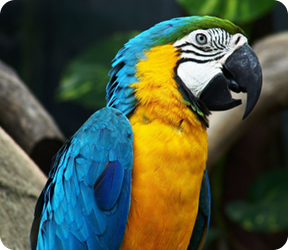
\includegraphics[width=0.9\textwidth]{figures/arara.png}\par}
%
%\vspace{.7em}
%
%\em Do you like araras? We do, specially our tool
%which shares the same name of this colorful bird.
%\end{minipage}\hspace{1em}
%\begin{minipage}{0.5\textwidth}
%The tool name was chosen as an homage to a Brazilian bird
%of the same name, which is a macaw. The word \emph{arara}
%comes from the Tupian word \emph{a'rara}, which means
%\emph{big bird} (much to my chagrin, Sesame Street's
%iconic character Big Bird is not a macaw; according
%to some sources, he claims to be a golden condor).
%Araras are colorful, noisy, naughty and very funny.
%Everybody loves araras. The name seemed catchy for a
%tool and, in the blink of an eye, \arara\ was quickly
%spread to the whole \TeX\ world.
%\end{minipage}
%\end{messagebox}
%
%Now that we informally introduced rules and directives,
%let us take a look on how \arara\ actually works given
%those two elements. The whole idea is pretty straightforward,
%and I promise to revisit these concepts later on in this manual
%for an comprehensive explanation.
%
%First and foremost, we need to add at least one instruction
%in the source code to tell \arara\ what to do. This
%instruction is named \emph{directive} and it will be parsed during the preparation phase. Observe that \arara\ will tell
%you if no directive was found in a file, as seen in our
%first interaction with the tool.
%
%An \arara\ directive is usually defined in a line of its
%own, started with a comment (denoted by \verb|%| in \TeX\ and
%friends), followed by the word \verb|arara:| and task name:
%
%\begin{codebox}{A typical directive}{teal}{\icnote}{white}
%% arara: pdflatex
%\documentclass{article}
%...
%\end{codebox}
%
%Our sample has one directive, referencing \verb|pdflatex|.
%It is important to observe that the \verb|pdflatex|
%identifier does not represent the command to be executed,
%but the name of the rule associated with that directive.
%
%\begin{messagebox}{New feature in version 4.0}{araracolour}{\icinfo}{white}
%\textbf{Multiline directives} -- Later on, we will discover
%that a directive can also span several lines in order to
%ease code writing. For now, a typical directive occupies
%only one line, even if spanning several columns.
%\end{messagebox}
%
%Once \arara\ finds a directive, it will look for the
%associated \emph{rule}. In our example, it will look for
%a rule named \verb|pdflatex| which will evidently run the
%\verb|pdflatex| command line application.
%
%\begin{messagebox}{New feature in version 4.0}{attentioncolour}{\icattention}{black}
%\textbf{REPL workflow} -- \arara\ now employs a REPL workflow
%for rules and directives. In previous versions, directives
%were extracted, their corresponding rules were analized,
%commands were built and added to a queue before any proper
%execution or evaluation. I decided to change this workflow,
%so now \arara\ evaluates each rule on demand, that is, there
%is no \emph{a priori} checking. A rule will \emph{always}
%reflect the current state, including potential side effects
%from previous executed rules. 
%\end{messagebox}
%
%Now, we have a queue of pairs $(\textit{directive}, \textit{rule})$ to process. For each pair, \arara\ will
%map the directive to its corresponding rule, evaluate it
%and run the proper command. The execution chain requires
%that command $i$ was successfully executed to then
%proceed to command $i+1$, and so forth. This is also by
%design: \arara\ will halt the execution if any of the
%commands in the queue had raised an error. How does one
%know if a command was successfully executed? \arara\
%checks the corresponding \emph{exit status} available
%after a command execution. In general, a successfull
%execution yields 0 as its exit status.
%
%\begin{messagebox}{New feature in version 4.0}{araracolour}{\icinfo}{white}
%\textbf{Custom exit status checking} -- In previous versions,
%there was no way of customizing the exit status checking of
%a command. A command was successful if, and only if, its
%resulting exit status was 0 and no other value. From now on,
%we can define any value, or even forget about it and make it
%always return a valid status regardless of execution (for
%instance, in a rule that always is successful).
%\end{messagebox}
%
%That is pretty much how \arara\ works: directives in the
%source code are mapped to rules. These pairs are added
%to a queue. The queue is then executed and the status is reported. We will cover more details about the expansion
%process later on in the manual. In short, we teach \arara\
%to do a task by providing a rule, and tell it to execute it
%through directives in the source code.
%
%\section{Operating system remarks}
%
%The application was written using the Java language, so
%\arara\ runs on top of a Java virtual machine, available
%on all the major operating systems~--~in some cases, you
%might need to install the proper virtual machine. We tried
%very hard to keep both code and libraries compatible with
%older virtual machines or from other vendors. Currently,
%\arara\ is known to run on Oracle's Java 5 to 10, and
%OpenJDK 5 to 10. I also have reports of users sucessfully
%using the tool with virtual machines provided by Azul
%Systems, so your mileage might vary.
%
%\begin{messagebox}{Outdated Java virtual machines}{warningcolour}{\icerror}{white}
%Dear reader, beware of outdated software, mainly Java virtual
%machines! Although \arara\ offers support for older virtual
%machines, try your best to keep your software updated as
%frequently as possible. The legacy support exists only for
%historical reasons, and also due to the sheer fact that I know
%some people that still runs \arara\ on very old hardware. If you
%are not in this particular scenario, get the latest virtual
%machine.
%\end{messagebox}
%
%Later on in this manual, we will provide instructions on
%how to build \arara\ from sources using Apache Maven. Even if
%you use multiple operating systems, \arara\ should behave the 
%same, including the rules. There are helper functions
%available in order to provide support for system-specific rules 
%based on the underlying operating system.
%
%\section{Support}
%
%If you run into any issue with \arara, please let us know.
%We all have very active profiles in the
%\href{https://tex.stackexchange.com/}{\TeX\ community at
%StackExchange}, so just use the \verb|arara| tag in your
%question and we will help you the best we can (also, take a
%look at their
%\href{https://tex.meta.stackexchange.com/q/1436}{starter guide}). 
%We also have a
%\href{https://gitter.im/cereda/arara}{Gitter chat room}, in which
%we occasionally hang out. Also, you if you think the report is 
%worthy of an issue, open one in our
%\href{https://github.com/cereda/arara/issues}{GitHub repository}. 
%At last, but not least, feel free to poke us by good old
%electronic mail (please try the other approaches first).
%
%I really hope you like my humble contribution to the \TeX\ 
%community. Let \arara\ enhance your \TeX\ experience, it will
%help you when you will need it the most. Enjoy the manual.
%
%\chapter{Important concepts}
%\label{chap:importantconcepts}
%
%Time for our first contact with \arara! I must strees that
%is very important to understand a few concepts in which
%\arara\ relies before we proceed to the usage itself.
%Do not worry, these concepts are easy to follow, yet they
%are vital to the comprehension of the application and the
%logic behind it.
%
%\section{Rules}
%
%A \emph{rule} is a formal description of how \arara\
%handles a certain task. For instance, if we want to use
%\verb|pdflatex| with our tool, we should have a rule for
%that. Directives are mapped to rules, so a call to a
%nonexistent rule \verb|foo|, for instance, will
%indeed raise an error:
%
%\begin{codebox}{Terminal}{teal}{\icnote}{white}
%$ arara doc1.tex
%  __ _ _ __ __ _ _ __ __ _ 
% / _` | '__/ _` | '__/ _` |
%| (_| | | | (_| | | | (_| |
% \__,_|_|  \__,_|_|  \__,_|
%
%Processing 'doc1.tex' (size: 83 bytes, last modified: 05/03/2018
%12:10:33), please wait.
%
%I could not find a rule named 'foo' in the provided rule paths.
%Perhaps a misspelled word? I was looking for a file named
%'foo.yaml' in the following paths in order of priority:
%(/opt/paulo/arara/rules)
%
%Total: 0.09 seconds
%\end{codebox}
%
%Once a rule is defined, \arara\ automatically provides an
%access layer to that rule through directives in the source
%code, a concept to be formally introduced in the following
%section. Observe that a directive reflects a particular
%instance of a rule of the same name.
%
%A rule is a plain text file written in the YAML format.
%I opted for this format because back then it cleaner
%and more intuitive to use than other markup languages,
%besides of course being a data serialization standard for programming languages.
%
%\begin{messagebox}{Animal jokes}{araracolour}{\icok}{white}
%As a bonus, the acronym \emph{YAML} rhymes with the word
%\emph{camel}, so \arara\ is heavily environmentally friendly.
%Speaking of camels, I could rewrite the tool in Perl, but I
%would rather not rage at my editor right now.
%\end{messagebox}
%
%The default rules, that is, the rules shipped with \arara, are
%placed inside a special subdirectory named \verb|rules/| inside
%\verb|ARARA_HOME|. We will learn later on that we can add an
%arbitrary number of paths for storing our own rules, in order
%of priority, so do not worry too much with the location of the
%default rules, although it is important to understand and
%acknowledge their existance. The basic structure of an
%\arara\ rule is:
%
%\begin{codebox}{Basic rule struture}{teal}{\icnote}{white}
%!config
%# Hello, I am a comment
%identifier: pdflatex
%name: PDFLaTeX
%commands:
%- name: PDFLaTeX engine
%  command: pdflatex @{file}
%arguments: []
%\end{codebox}
%
%Let us break down the structure into parts, so it will be easier for us to grasp the elements, hopefully. The indices correspond to the line numbering scheme in the previous code.
%
%\begin{linedescription}
%\item The \verb|!config| keyword is mandatory and must be
%the first line of any \arara\ rule. It denotes the object
%mapping metadata to be internally used by the tool. 
%
%\item A comment line starts with the \verb|#| symbol.
%
%\item The \verb|identifier| key acts as a unique identifier
%for the rule (as expected). It is highly recommended to use
%lowercase letters without spaces, accents or punctuation symbols.
%As a convention, if you have an identifier named \verb|pdflatex|,
%the rule filename must be \verb|pdflatex.yaml| (like our own
%instance).
%
%\item The \verb|name| key holds the name of the task. When
%running \arara, this value will be displayed in the output.
%In our example, the tool will display \verb|PDFLaTeX| as task
%name in the output when dealing with this task. Task names are
%displayed enclosed in parenthesis.
%
%\item The \verb|commands| key is introduced in version 4.0 of
%\arara\ and denotes a potential list of subtasks. A task may
%represent only a single command, as well as a sequence of
%commands (for example, the \verb|frontespizio| rule requires
%at least two commands). So, as a means of normalizing the
%representation, a task composed of a single command (like
%the one in our example) is defined as the only element
%of such list. The keys used inside this list specification
%are defined as follows. A list element is denoted by \verb|-|
%(hyphen).
%
%\item The \verb|name| key has no relation with the previously
%presented key of the same name. In this specific context,
%this key holds the subtask name. When running \arara\, this
%value will be displayed in the output right after the
%task name.
%
%\item The \verb|command| key contains the system command to be
%executed. You can use virtually any type of command,
%interactive or noninteractive. But beware: if \arara\ is
%running in silent mode, which is the default behaviour,
%an interactive command wich might require the user
%input will be halted and the execution will fail.
%Do not despair, you can use a special \verb|--verbose|
%flag with \arara\ in order to interact with such
%commands -- we will talk about flags later on. You probably
%noticed a strange element \verb|@{file}| in the
%\verb|command| line: this element is called \emph{orb tag}.
%For now, just admit these elements exist. We will come back
%to them later on, I promise.
%
%\item The \verb|arguments| key denotes a list of arguments
%for the subtask command. In our example, we have an empty
%list, denoted by \verb|[]|. You can define as many arguments
%as your subtask requires.
%\end{linedescription}
%
%For more complex rules, we might want to use arguments.
%The following code presents a new rule which makes use
%of them instead of an empty list as the previous code:
%
%\begin{codebox}{Adding rule arguments}{teal}{\icnote}{white}
%!config
%identifier: copy
%name: Copy
%commands:
%- name: Copy operation
%  command: copy @{from} @{to}
%arguments:
%- identifier: from
%  flag: '@{parameters.from}'
%- identifier: to
%  flag: '@{parameters.to}'
%\end{codebox}
%
%For every argument in the \verb|arguments| list, we have a
%\verb|-| mark (hyphen) and proper indentation. Let us break down the relevant parts of this new rule:
%
%\begin{linedescription}[start=8]
%\item The \verb|identifier| key acts as a unique identifier
%for the current argument. It is highly recommended to use
%lowercase letters without spaces, accents or punctuation
%symbols.
%
%\item The \verb|flag| key represents the argument value.
%Note that we have other orb tags in the argument
%definitions, \verb|@{parameters.from}| and
%\verb|@{parameters.to}|; we will discuss them later on. Just
%to give some context, \verb|parameters| is a special variable
%which maps the elements available in the directive being
%evaluated. For example, if we have \verb|from: a| in a
%directive, \verb|parameters.from|  will resolve to \verb|a|.
%The argument \verb|flag| value is only applied if, and only
%if, there is an explicit directive argument. Say, if
%\verb|from| is not defined as a directive argument, the
%\verb|flag| value of argument \verb|from| will be
%resolved to an empty string.
%\end{linedescription}
%
%\begin{messagebox}{Overriding the default resolution of nonexistent arguments}{araracolour}{\icinfo}{white}
%If a certain argument does not exist in the directive, its
%rule counterpart will be resolved to an empty string, as the
%default resolution. As a means to overriding this behaviour
%when a directive argument is not specified, use the \verb|default| key within the argument specification.
%\end{messagebox}
%
%When a rule argument just needs a default value regardless of
%a user-specified value, you can safely ignore the \verb|flag|
%key and rely on the \verb|default| one. Similarly, if you need
%to map a directive argument into a rule argument without falling 
%back to a default value different than an empty string, 
%just use the \verb|flag| key. Now, if you need mapping and 
%fallback, stick with both keys. Just keep in mind that at least 
%one of them must exist!
%
%\begin{messagebox}{New feature in version 4.0}{araracolour}{\icinfo}{white}
%\textbf{Required arguments} -- Sometimes, we might end up with
%a rule in need of mandatory arguments. For instance, the
%two arguments of our \verb|copy| should be mandatory, as it makes
%no sense to have optional values for a copy operation. In this
%case, add a \verb|required| key to the relevant argument and set 
%the corresponding value to \verb|true| (a boolean value). Setting
%such value to \verb|false| would fallback to the default
%behaviour.
%\end{messagebox}
%
%All subtasks in a rule are checked against their corresponding
%exit status. If an abnormal execution is detected, \arara\ will
%instantly halt.
%
%For now, we need to keep in mind that \arara\ uses rules to tell
%it how to do a certain task (and subtasks). In the next sections,
%when more concepts are presented, we will come back to this
%subject. Just a taste of things to come, as we mentioned before
%already: directives are mapped to rules through orb tags. Do not
%worry, I will explain how things work.
%
%\begin{messagebox}{There are better ways of writing a rule}{attentioncolour}{\icattention}{black}
%This section covered the simplest way of writing an \arara\ rule,
%solely for didactic (and also historical) reasons. Keep in mind that there are far better and ways to achieve consistent rules. We
%need to discuss more about the basics before entering into
%advanced topics.
%\end{messagebox}
%
%\section{Directives}
%\label{sec:directives}
%
%A \emph{directive} is a special comment inserted in the
%source file in which you indicate how \arara\ should
%behave. You can insert as many directives as you
%want and in any position of the file. The tool will
%read the whole file and extract the directives.
%
%\begin{messagebox}{New features in version 4.0}{araracolour}{\icinfo}{white}
%\textbf{Partial directive extraction} -- From version 4.0 on,
%it is now possible to extract directives only available in the
%file preamble, that is, all lines from the beginning that are
%comments until reaching the first line that is not a comment.
%To this end, a new command line flag is introduced. We will
%discuss this feature later on.
%
%\vspace{1em}
%
%\textbf{Predefined preambles} -- It is now possible to set up
%a common preamble to be used with files that require the same
%automation steps, then \arara\ can be invoked based on such
%specifications. We will discuss this feature later on.
%\end{messagebox}
%
%There are two types of directives in \arara. The first one has
%already been mentioned, it has only the rule name (which refers 
%to the \verb|identifier| key from the rule of the same name). It 
%is called \emph{empty directive}:
%
%\begin{codebox}{Empty directive}{teal}{\icnote}{white}
%% arara: pdflatex
%\end{codebox}
%
%Sometimes, however, we need to provide additional information to 
%the rule. That is reason for the second type, the 
%\emph{parametrized directive}, to exist. As the name indicates, 
%we have directive arguments! They are mapped by their identifiers
%and not by their positions. The syntax for a parametrized 
%directive is:
%
%\begin{codebox}{Parametrized directive}{teal}{\icnote}{white}
%% arara: pdflatex: { shell: yes }
%\end{codebox}
%
%Each argument is defined according to the rule mapped by the 
%directive. This means you cannot use an argument \verb|foo| in a 
%directive \verb|bar| if the rule \verb|bar| does not offer 
%support for it (that is, \verb|bar| has to have \verb|foo| 
%defined as argument in its list of arguments inside the rule 
%scope, as seen in the previous section). The syntax for
%an argument is:
%
%\begin{codebox}{Argument syntax}{teal}{\icnote}{white}
%key : value
%\end{codebox}
%
%Suppose we would like to enable shell escape for \verb|pdflatex| 
%when compiling a \verb|hello.tex| file. We can achieve that by 
%providing a parametrized directive, like this one:
%
%\begin{codebox}{\texttt{hello.tex} with a parametrized directive}{teal}{\icnote}{white}
%% arara: pdflatex: { shell: yes }
%
%\documentclass{article}
%\begin{document}
%Hello world!
%\end{document}
%\end{codebox}
%
%Of course, the \verb|shell| argument is defined in the
%\verb|pdflatex| rule scope, otherwise \arara\ would raise
%an error about an invalid argument key. If we try to
%inject a nonexistent \verb|foo| argument in the previous 
%parametrized directive, we will get this message:
%
%\begin{codebox}{Terminal}{teal}{\icnote}{white}
%  __ _ _ __ __ _ _ __ __ _ 
% / _` | '__/ _` | '__/ _` |
%| (_| | | | (_| | | | (_| |
% \__,_|_|  \__,_|_|  \__,_|
%
%Processing 'hello.tex' (size: 103 bytes, last modified:
%05/03/2018 15:40:16), please wait.
%
%I have spotted an error in rule 'pdflatex' located at
%'/opt/paulo/arara/rules'. I found these unknown keys
%in the directive: (foo). This should be an easy fix,
%just remove them from your map.
%
%Total: 0.21 seconds
%\end{codebox}
%
%As the message suggests, we need to remove the unknown argument 
%key from our directive or rewrite the rule in order to include 
%it. The first option is, of course, easier.
%
%\begin{messagebox}{Helpful messages}{araracolour}{\icinfo}{white}
%Make sure to read all messages \arara\ raises, they will help 
%you!
%\end{messagebox}
%
%Sometimes, directives can span several columns of a line, 
%particularly the ones with several arguments. From \arara\ 4.0 
%on, we can split a directive into multiple lines by adding
%\verb|% arara: -->| to each line which should compose the
%directive:
%
%\begin{codebox}{Multiline directive}{teal}{\icnote}{white}
%% arara: pdflatex: {
%% arara: --> shell: yes,
%% arara: --> synctex: yes
%% arara: --> }
%\end{codebox}
%
%It is important to observe that there is no need of them to be
%in contiguous lines, that is, provided that the syntax for
%parametrized directives hold for the line composition, lines can
%be distributed all over the code.
%
%\begin{messagebox}{New feature in version 4.0}{araracolour}{\icinfo}{white}
%\textbf{Conditionals} -- From version 4.0 on, \arara\ provides
%logical expressions processed at runtime to determine whether
%and  how a directive should be processed. This is a huge 
%improvement towards better user experience.
%\end{messagebox}
%
%One of the most awaited features that version 4.0 introduces is 
%the support of conditionals, that is, logical expressions 
%processed at runtime in order to determine whether and how the 
%directive should be processed. The following types are allowed:
%
%\begin{keywords}
%\item[if] evaluated beforehand, the directive is interpreted
%if and only if the result is true.
%
%\item[unless] evaluated beforehand, the directive
%is interpreted if and only if the result is false.
%
%\item[until] directive is interpreted the first time,
%then the evaluation is done; while the result
%is false, the directive is interpreted again and
%again.
%
%\item[while] evaluated beforehand, the directive is
%interpreted if and only if the result is true,
%and the process is repeated while the result
%still holds true.
%\end{keywords}
%
%We will discuss this special feature later on, including methods
%available in the directive scope in order to ease the writing
%of conditionals, as it would be highly advisable to have
%orb tags covered beforehand.
%
%\section{Orb tags}
%\label{sec:orbtags}

\end{document}
